\documentclass[xcolor={dvipsnames}, aspectratio=169]{beamer}
\usetheme{Darmstadt}
\usecolortheme{dolphin}
\usepackage[logic, complexity, graphs]{commondefns}
\usefonttheme[onlymath]{serif}
\usepackage{csquotes}
\usepackage[style=alphabetic]{biblatex}
\addbibresource{refs.bib}
\usepackage{bussproofs}

%\includeonlyframes{current}

\title{Lower Bounds for the Polynomial Calculus\\via the ``Pigeon Dance''}
\author{Imogen Hergeth}
\date{January 2023}
\setbeamertemplate{navigation symbols}{
    \usebeamerfont{footline}\insertframenumber / \inserttotalframenumber
}


\newcommand{\Sn}{S_n(\KK)}
\newcommand{\Snd}{S_{n, d}(\KK)}
\newcommand{\PHP}{\ensuremath{\neg \mathcal{PHP}^m_n}\xspace}
\newcommand{\Qiij}{Q_{i_1, i_2, j}}
\newcommand{\LT}{\operatorname{LT}}
\newcommand{\Rsem}{R^\mathrm{sem}}
\newcommand{\Rsyn}{R^\mathrm{syn}}
\newcommand{\Dsem}{\Delta^\mathrm{sem}}
\newcommand{\Dsyn}{\Delta^\mathrm{syn}}
\newcommand{\fa}{\text{ for all }}
\renewcommand{\K}{\operatorname{Kill}}
\newcommand{\Is}{{I \setminus \{i_1\}}}
\newcommand{\rhoij}{\rho_{i_1 j_1}}
\newcommand{\xij}{{x_{i_1 j_1}}}

\definecolor{amaranth}{rgb}{0.9, 0.17, 0.31}
\definecolor{pastelred}{rgb}{1.0, 0.41, 0.38}
\definecolor{plum}{rgb}{0.56, 0.27, 0.52}

\definecolor{emerald}{rgb}{0.31, 0.78, 0.47}
\definecolor{caribbeangreen}{rgb}{0.0, 0.8, 0.6}
\definecolor{darkcyan}{rgb}{0.0, 0.55, 0.55}
\definecolor{darkpastelgreen}{rgb}{0.01, 0.75, 0.24}
\definecolor{saffron}{rgb}{0.96, 0.77, 0.19}
\definecolor{chromeyellow}{rgb}{1.0, 0.65, 0.0}
\definecolor{darkorange}{rgb}{1.0, 0.55, 0.0}

\definecolor{bleudefrance}{rgb}{0.19, 0.55, 0.91}

\colorlet{deltaCol}{amaranth}
%\colorlet{Rcol}{bleudefrance}
\colorlet{Vcol}{bleudefrance}
\colorlet{reqCol}{saffron}

\begin{document}
\maketitle

\section{Introduction}

\begin{frame}{Overview}
    We will present the result from A.A. Razborov, ``Lower Bounds for the Polynomial Calculus'',
    in: Computational Complexity 7.4 (Dec. 2, 1998).

    \tableofcontents[hideallsubsections]
\end{frame}

\subsection{The polynomial calculus}

\begin{frame}{Background}
    \begin{itemize}[<+->]
        \item Lower bounds for proofs in various systems
        \item In particular for the pigeonhole principle
        \item Polynomial calculus is a strong proof system
        \item Provide a lower bound for it with the pigeonhole principle
    \end{itemize}
\end{frame}

\begin{frame}{Definition}
    \begin{itemize}[<+->]
        \item Similar to sequent calculus, but lines are polynomials
        \item We use multilinear polynomials $S(\KK)$\\
            ($xy + xz + v \equiv x^2y + x^3z^5 + v$)
        \item Addition
        \begin{prooftree}
            \AxiomC{$f$}
            \AxiomC{$g$}
            \BinaryInfC{$af + bg$}
        \end{prooftree}
        \item Multiplication
        \begin{prooftree}
            \AxiomC{$f$}
            \UnaryInfC{$f \cdot x$}
        \end{prooftree}
    \end{itemize}
\end{frame}

\begin{frame}{Refutations}
    \begin{itemize}[<+->]
        \item $g$ is provable from $f_1, \ldots, f_n$ if and only if it is in the ideal generated by them
        \item A proof of $1$ exists if and only if $f_1, \ldots, f_n$ have no common zeroes
        \item We construct polynomials such that their zeroes correspond to satisfying assignments
        \item Proving $1$ from them is a \textit{refutation}
    \end{itemize}
\end{frame}

\begin{frame}{Example proof}
    \begin{itemize}[<+->]
        \item Try to prove $xy + z$ from $x + 1$ and $z$
    \end{itemize}
    \uncover<+->{
    \begin{prooftree}
        \AxiomC{$x+1$}
        \only<-.>{\noLine}
        \LeftLabel{\uncover<+->{$(\cdot y)$}}
        \UnaryInfC{\uncover<.->{$xy + y$}}
        \AxiomC{\uncover<+->{$z$}}
        \only<-3>{\noLine}
        \RightLabel{\uncover<.->{$(+)$}}
        \BinaryInfC{\uncover<.->{$xy + y + z$}}
    \end{prooftree}
    }
    \begin{itemize}[<+->]
        \item We now want to subtract $y$
        \item There is no way to prove $y$ from $x+1$ and $z$
        \item Closest to $xy + z$ we can prove is $xy + y + z$
    \end{itemize}
\end{frame}

\begin{frame}{Algebraic view of proofs}
    \begin{itemize}[<+->]
        \item Think of polynomials not just as lines but as elements of \KK-algebras
        \item $\textcolor{Vcol}{V}$ are polynomials we can prove \hfill \textcolor{Vcol}{$xy + y + z$}
        \item $\textcolor{deltaCol}{\Delta}$ are leading terms of ones we cannot prove \hfill \textcolor{deltaCol}{$y$}
        \item $S(\KK) \cong \KK \textcolor{deltaCol}{\Delta} \oplus \textcolor{Vcol}{V}$ \hfill $xy + z = -\textcolor{deltaCol}{y} + \textcolor{Vcol}{xy + y + z}$
        \item Similarly $\textcolor{Vcol}{V_d}, \textcolor{deltaCol}{\Delta_d}$ for proofs of bounded degrees
        \item Investigate what $\textcolor{Vcol}{V_d}$ looks like
    \end{itemize}
\end{frame}

\section{The Pigeonhole Principle}
\subsection{Overview}
\begin{frame}{The pigeonhole principle}
    \begin{itemize}[<+->]
        \item If there are $m$ pigeons, $n$ pigeon holes, and $m > n$ then at least two pigeons have to share a hole
        \item Formally: if $m > n$ there is no injection $[m] \tomono [n]$
        \item Variables: $x_{i j}, i \in [m], j \in [n]$
        \item Assignment of $x_{3, 5}$ corresponds to pigeon $3$ being in hole $5$
    \end{itemize}
    \begin{definition}<+->[\PHP]
        \begin{align*}
            Q_i &\coloneqq 1 - \sum_{j \in [n]} x_{ij} &&\text{for each $i \in [m]$}\\
            \Qiij &\coloneqq x_{i_1j} x_{i_2j} &&\text{for each $i_1 \neq i_2 \in [m], j \in [n]$}
        \end{align*}
    \end{definition}
\end{frame}

\begin{frame}{Main result}
    \begin{theorem}<+->
        Every polynomial calculus refutation of \PHP must have degree at least $n/2 + 1$.
    \end{theorem}
    \begin{itemize}[<+->]
        \item Goal: if $d < n/2 + 1$, then $1 \not\in \textcolor{Vcol}{V_d} \Leftrightarrow \textcolor{Vcol}{V_d} \neq S(\KK)$
        \item Characterize $\textcolor{Vcol}{V_d}$ in a way that lets us see this
        \item Prove this characterization is correct via the pigeon dance
    \end{itemize}
\end{frame}

\begin{frame}{\PHP constraints}
    \begin{itemize}[<+->]
        \item Polynomials in \PHP are constraints on assignments
        \item Inference rules preserve constraints
        \item Pigeons cannot share holes
        \item Possible for pigeons $I \subseteq [m]$ with $|I| \leq n$
        \item Locally valid assignments are injections $I \tomono [n]$
        \item Corresponding variable assignments are $M_I$
    \end{itemize}
\end{frame}

\begin{frame}{Locally valid assignments}
    \begin{itemize}[<+->]
        \item Define $\textcolor{Vcol}{V_I}$ as the set of all polynomials with $a(f) = 0$ for all $a \in M_I$
        \item Claim: $\textcolor{Vcol}{V_d} = \bigcup_{|I| \leq d} V_I$
        \item Clearly $a(1) \neq 0$ for all $a \in M_I, I \subseteq [m]$
        \item This definition completely ignores the degrees of the proofs!
        \item Only works if for all terms $t$, $t \in \textcolor{deltaCol}{\Delta_I}$ for either all or no $I \supseteq \dom(t)$
    \end{itemize}
\end{frame}

\section{The Pigeon Dance}
\subsection{Ideas}

\begin{frame}{Overview}
    \begin{itemize}[<+->]
        \item Goal:
            \begin{itemize}[<.->]
                \item Use pigeon dance to characterize $\textcolor{deltaCol}{\Delta_I}$
                \item Prove correctness
            \end{itemize}
        \item Start with pigeons sitting in their holes
        \item The first pigeon flies to an unoccupied hole to its right
        \item Repeat until all pigeons have moved once
        \item If a pigeon cannot find an empty hole, the dance is aborted
    \end{itemize}
\end{frame}

\newcommand{\pigeon}[3]{
    \node#3 (pigeon#1) at (#2, 1) [label={[label distance=-.8cm]-145:#1}]
        {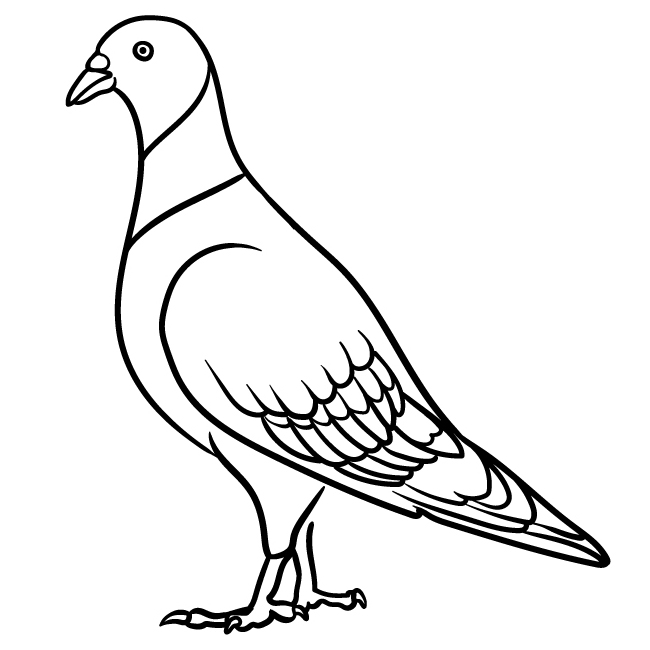
\includegraphics[width=1.5cm]{pigeon.jpg}};
}

\newcommand{\flight}[3]{
    \node#3 (flight#1) at (#2, 3.2) [label={[label distance=-.8cm]-145:#1}]
        {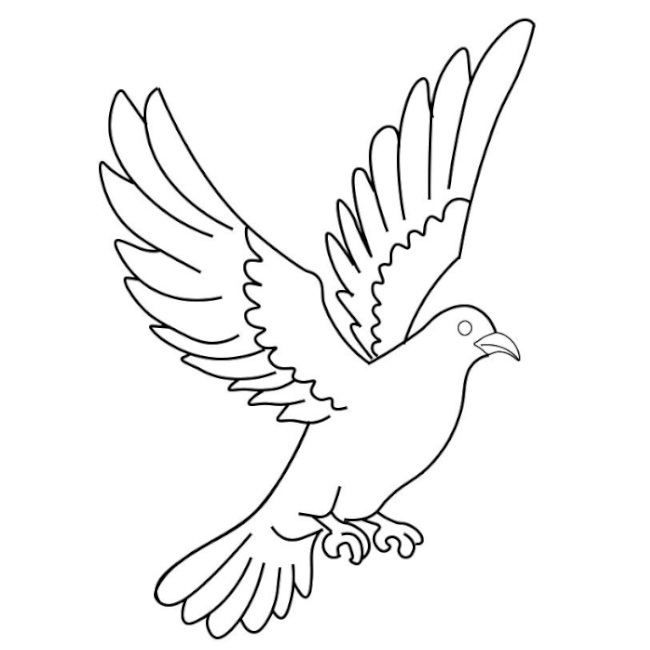
\includegraphics[width=1.5cm]{flight.jpg}};
}

\begin{frame}[label=current]{Example}
    \centering

    \begin{tikzpicture}
        \path (-1, 4.7) -- (13, 4.7);
        \draw[draw=black] (0, 0) rectangle ++(2, 2);
        \draw[draw=black] (2.5, 0) rectangle ++(2, 2);
        \draw[draw=black] (5, 0) rectangle ++(2, 2);
        \draw[draw=black] (7.5, 0) rectangle ++(2, 2);
        \draw[draw=black] (10, 0) rectangle ++(2, 2);

        \pigeon{1}{8.5}{<+>}
        \pigeon{2}{1}{<.-3>}
        \pigeon{3}{3.5}{<.-5>}
        \flight{1}{9.75}{<+>}
        \pigeon{1}{11}{<+->}
        \flight{2}{4.75}{<+>}
        \pigeon{2}{8.5}{<+->}
        \flight{3}{4.75}{<+>}
        \pigeon{3}{6}{<+->}
    \end{tikzpicture}
\end{frame}

\begin{frame}{Formalization}
    \begin{itemize}[<+->]
        \item Consider partial injections $I \tomono [m]$ \qquad ($1 \mapsto 4, \enspace 2 \mapsto 1, \enspace 3 \mapsto 2$)
        \item Encode pigeon positions as terms \qquad (\textcolor{deltaCol}{$x_{1, 4} \, x_{2, 1} \, x_{3, 2}$})
        \item $\textcolor{deltaCol}{\Delta_I}$ is the set of terms that let pigeons complete the dance
        \item Membership in $\textcolor{deltaCol}{\Delta_I}$ is independent of $I$ since pigeons not in the dance do not affect it
    \end{itemize}
\end{frame}

\subsection{Properties}
\begin{frame}{The $\K$ operator}
    \begin{itemize}[<+->]
        \item We need to further understand the dance to prove it correct
        \item Idea: a way to block specific pigeon holes
        \item Kill the first pigeon and moves its hole to the left
        \item $\K(x_{i_1 j_1} \cdots x_{i_d, j_d}) = x_{i_2 j'_2} \cdots x_{i_d j'_d}$ with\\
            $$j'_k \coloneqq \begin{cases}
                    j_k + 1, &\text{if } j_k < j_1\\
                    j_k, &\text{if } j_k > j_1.
                \end{cases}$$
    \end{itemize}
\end{frame}

\begin{frame}{Simulating the pigeon dance with $\K$}
    \stepcounter{beamerpauses}
    \begin{theorem}<+->
        $x_{i_1 j_1} \cdots x_{i_d j_d} \in \textcolor{deltaCol}{\Delta_I}$ if and only if there is a $j' > j_1$ such that
        $\K(x_{i_1 j'} \cdots x_{i_d j_d}) \in \textcolor{deltaCol}{\Delta_I}$.
    \end{theorem}
    \begin{proof}[Proof sketch\nopunct]<+->
        $\K(x_{i_1 j'} \cdots x_{i_d j_d})$ effectively moves the first pigeon to an empty hole to its right and then kills it.
        This is the same as each step in the dance, where the first pigeon flies to some free hole to its right and then occupies it.
    \end{proof}
\end{frame}

\begin{frame}{Closure of $\textcolor{deltaCol}{\Delta_I}$}
     \begin{theorem}<+->
        $\textcolor{deltaCol}{\Delta_I}$ is closed under $\K$.
     \end{theorem}
    \begin{proof}[Proof sketch\nopunct]<+->
        If $t \in \textcolor{deltaCol}{\Delta_I}$ then the pigeons can complete their dance. During this the first pigeon will start at
        $j$ and fly to $j'$. Killing the pigeon frees up $j'$ so any other pigeon that wanted to use $j$ can use it instead.
    \end{proof}
\end{frame}

\begin{frame}{The lower bound}
    \begin{theorem}<+->
        If $|I| \leq (n+1) / 2$ and $t \in \textcolor{deltaCol}{\Delta_I}$, then there is a hole $j$
        such that $\K(x_{ij} t) \in \textcolor{deltaCol}{\Delta_I}$.
    \end{theorem}
    \begin{proof}[Proof sketch\nopunct{}]<+->
        There are at most $$
            |\dom(t)| \leq |I \setminus \{i\}| \leq \frac{n - 1}{2}
        $$ pigeons involved in the dance, each occupying two holes. Place pigeon at unused hole and kill it there.
        The remaining pigeons can complete the dance since the moved hole was not used.
    \end{proof}
\end{frame}

\section{Conclusion}

\begin{frame}{Putting things together}
    \begin{itemize}[<+->]
        \item Goal: show pigeon dance correctly characterizes $S(\KK) / \textcolor{Vcol}{V_I}$
        \item In particular: each $f \in \KK \textcolor{deltaCol}{\Delta_I}$ has an $a \in M_I$ with $a(f) \neq 0$
        \item Induction over $|I|$
        \item Remove variables $x_{ij}$ for minimal $i \in I$ from $f$
        \item Inductive assumption gives us $a' \in M_{I\setminus \{i\}}$ with $a'(f') \neq 0$ \hfill \textcolor{reqCol}{closure of $\textcolor{deltaCol}{\Delta_I}$}
        \item Pick a $j$ such that $\K(x_{i j} t) \in \textcolor{deltaCol}{\Delta_I}$   \hfill \textcolor{reqCol}{lower bound}
        \item Extend assignment to $I$ with $a(f) \neq 0$
    \end{itemize}
\end{frame}

\begin{frame}{Summary}
    \begin{itemize}[<+->]
        \item Proven a lower bound $d \geq n/2 + 1$ for polynomial calculus refutations of \PHP
        \item Characterize derivable polynomials \textcolor{Vcol}{$V_d$} through locally consistent assignments $M_I$
        \item This only works if membership in $\textcolor{deltaCol}{\Delta_I}$ is independent of $I$
        \item Characterize $\textcolor{deltaCol}{\Delta_I}$ through pigeon dance
        \item Correct since $\textcolor{deltaCol}{\Delta_I}$ is linearly independent over $M_I$
    \end{itemize}
\end{frame}

\end{document}